% generated by plots/fig2_coalition.py --- do not edit the numbers by hand
% figure* --- the chapter is two-column and this does not fit one
\begin{figure*}[tp]
\centering
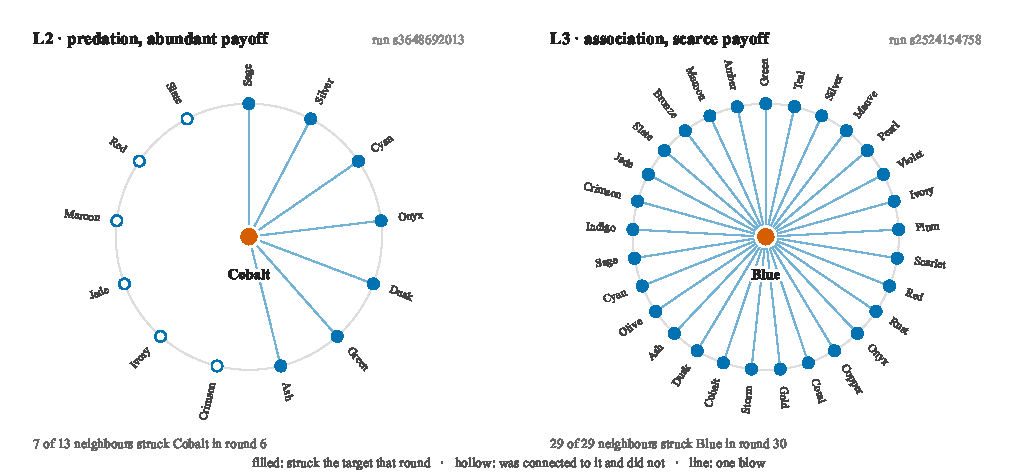
\includegraphics[width=\linewidth]{figures/fig2_coalition/coalitions.pdf}\\[2pt]
\caption[The largest attack each capacity level produced]{%
\textbf{The largest attack each capacity level produced.} The largest coalition each capacity level produced anywhere in the run set, drawn as the graph around the agent it struck. The target is at the centre and every agent connected to it that round is on the ring, filled where it joined the blow and hollow where it did not, with a line for each attacker. Attackers are placed first and abstainers after them, so the ring is not the graph's own layout and ties between two neighbours are not drawn. The two scenes are 7 of 13 at L2 abundant in round 6 of run \texttt{s3648692013}; 29 of 29 at L3 scarce in round 30 of run \texttt{s2524154758} \meth{m:many-attack-once}.}
\label{fig:coalition}
\end{figure*}
